\section{System's Perspective}
  \subsection{System Design}
  The developed MiniTwit system is complex and consists of many subsystems, each of which required a significant amount of decisions to construct.
  In this subsection we will describe the design of our system as a whole, including the rationale behind some of the decisions we have made during this project.
  \newline
  For the sake of clarity, we will dissect our system into different layers: frontend, API and data persistence.
  \begin{enumerate}
    \item Frontend\newline
    The frontend of our system is what provides users access to our system through a web interface, which is developed using Blazor (wasm) and C\#, as well as html and css.
    With blazor we are able to have our C\# code compiled to webassembly and executed natively in the client browser.
    The frontend communicates with our api using HTTP requests, containing json payloads of serialized or deserialized data.
    .........................

    \item API\newline
    The REST API is developed using ASP.NET and exposes endpoints for communicating with the MiniTwit service. 
    This includes execution of actions like following and unfollowing, as well as data fetching like feeds or user profiles.
    The API translates frontend HTTP calls into data manipulations using Entity Framework for ORM with a code-first approach.
    This allows us to focus on code first and automatically construct relational database schemas based on the relations between objects in our C\# code, managed by database migrations.
    .........................

    \item Data Persistence\newline
    For data persistence we use use multiple difference database management systems. 
    MiniTwit data such as users, followers and messages are stored in a postgres relational database, which integrates well with Entity Framework.
    Logging data are stored in an ElasticSearch database configured with lifetime policies to keep the size under control.
    Lastly we use RabbitMQ for temporarily storing user private messages in message queues, interfaced by MQTT over WS, to allow direct communication from our blazor frontend.
    ..................

  \end{enumerate}

  \subsection{System Architecture}
  Our system as a whole consists of 3 servers and a load balancer, all of which are hosted on digital ocean.
  Each server is running an NGINX server, which has been configured to serve as a reverse proxy for routing of subdomain access, e.g. master.pythonkindergarten.tech, slave.pythonkindergarten.tech, monitor.pythonkindergarten.tech etc.
  \newline
  Below is an overview of the 3 servers, as well as their function and purpose within our system.\newline
  
  \begin{enumerate}
    \item Master Server\newline
    The Master server is the master node in our Docker swarm and is responsible for maintaining cluster state, as well as managing service updates within the swarm.
    This server also hosts our Prometheus and Grafana containers, which were described in the monitoring section.
    \item Worker Server\newline
    The Worker server simply contributes to the pooled resources within our swarm. 
    It is a Docker swarm worker node, which runs multiple replicas of our service, hosting both API and frontend.

    \item Database Server\newline
    The Database server has multiple purposes, all of which relates to data persistence.
    This server hosts our Postgres database, which is our primary means of persistence within the system. 
    \newline
    It also hosts our logging system, which consists of an ElasticSearch database (for log persistence), as well as Kibana for visualization of the collected logs.
    \newline
    Lastly, it hosts our RabbitMQ broker.
    \item Load Balancer\newline
    The load balancer is hosted on Digital Ocean and allows us to balance incoming traffic on pythonkindergarten.tech between each of our docker swarm servers.
  \end{enumerate}
  \subsubsection{System Deployment}
  Deploment of our system as a whole has been partially automated using 'Insert Technology', such that a simple shell script will deploy most of our system architecture.
  The only parts not included in this automated system deployment are: something, something, something and something, due to the high setup/configuration complexity.

  All dependencies of your ITU-MiniTwit systems on all levels of abstraction and development stages. (That is, list and briefly describe all technologies and tools you applied and depend on.)
  
  \subsection{Subsystem interactions}
  There are many important subsystems (described in previous sections), collectively making the system work as a whole.
  In this section we will illustrate the most important interactions between these services, as seen in the diagram below.\newline
  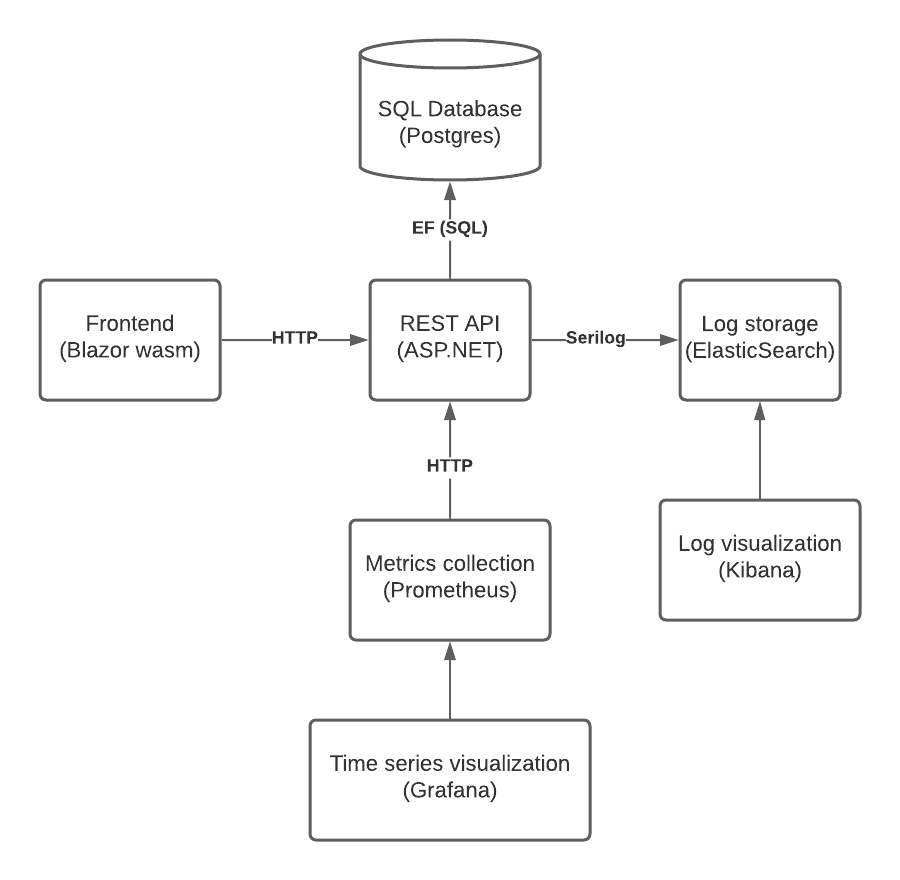
\includegraphics{images/InteractionDiagram.png}
\subsection{Dependencies}
Below is a list of all the \textbf{dependencies} of the Pythonkindergarten MiniTwit project, classified by description:
\begin{itemize}
    \item \textbf{Language, Runtimes, Templates and Dependency Manager:}
      .Net 5.0, ASP.Net Runtime 5.0, Blazor WebAssembly, WASM, NuGet
    \item \textbf{Project Structure:} Server, Client, Shared, Tests
    \item \textbf{Database:} Postgres, EntityFramework Core, EntityFramework NPSQL
    \item \textbf{Testing:} Xunit
    \item \textbf{Repository and Distributed Version Control:} Github, Git
    \item \textbf{Domain names and Domain service:} Pythonkindergarten.tech, .Tech Domains
    \item \textbf{DataTransferring over HTTP} JSON, System.Text.Json
    \item \textbf{Containerization:} Docker, Docker-Compose, DockerHub
    \item \textbf{Pipelines (CI/CD):} Github Actions (N.B. was initially Travis until migration to Github Actions)
    \item \textbf{Deployment Provider:} DigitalOcean
    \item \textbf{Server Certificate for application:} ZeroSSL
    \item \textbf{Monitoring Tools:} Prometheus, Grafana
    \item \textbf{Virtualization:} Vagrant
    \item \textbf{Logging:} Elasticsearch, Serilog, Kibana
    \item \textbf{Static Codecheck Tools:} SonarScanner, SonarCloud, CodeQL
    \item \textbf{Messaging:} RabbitMQ
\end{itemize}




\subsection{Describe the current state of your systems, for example using results of static analysis and quality assessment systems}
We use two different code analysis tools. 
They are both run in our CI pipeline. 
The first one is SonarCloud. The C\# Webassembly project and the API project are both analysed. 
The current state is that our test coverage is ~50\%. Which is below both the groups expection and Sonar clouds default expectation. 
Which is 90\% and 80\% respectively. 
Other than that a lot of informational messages are present. 

This is due to a static code analysis tool called Roslynator, which we wanted to analyze and refactor code smells.Then there are a few informational security messages, which have been looked through however they do not need to be acted on. There are also reports on "bad" exception handling, for example throwing general exception objects.The second tool we use, is called CodeQL. It is used to assess the security of our project. For example hard coded credentials or other vulnerable data, which must not be open to the public. It has not found anything of concern, only false positives, in our testing suite.

\subsection{Finally, describe briefly, if the license that you have chosen for your project is actually compatible with the licenses of all your direct dependencies.}
